% ============================================================================
%  End-of-internship progress report -- Hanoi urban noise
%
%  Build:  latexmk -pdf internship_report.tex
%
%  Every quantitative claim in this file is traceable to an artefact in the
%  repository, named at the point of use. Figures are copied from
%  deliverables/figures/, itself produced by scripts/12_presentation_figures.py
%  and scripts/08_validate_simulation.py. Anything not established by the
%  repository is marked [TO CONFIRM: ...] and listed again in Appendix A.
% ============================================================================
\documentclass[11pt,a4paper]{article}

\usepackage[T1]{fontenc}
\usepackage[utf8]{inputenc}
\usepackage[english]{babel}
\usepackage{lmodern}
\usepackage{microtype}
\usepackage[margin=25mm,headheight=14pt]{geometry}
\usepackage{array}
\usepackage{booktabs}
\usepackage{longtable}
\usepackage{graphicx}
\usepackage{xcolor}
\usepackage{amsmath}
\usepackage[round,authoryear]{natbib}
\usepackage{fancyhdr}
\usepackage{enumitem}
\usepackage{caption}
\usepackage[hidelinks]{hyperref}

\graphicspath{{figures/}}

\definecolor{ink}   {HTML}{1A1A1A}
\definecolor{accent}{HTML}{1F5C8B}
\definecolor{warnc} {HTML}{8A4B08}
\definecolor{grayc} {HTML}{6E6E6E}

\hypersetup{colorlinks=true, linkcolor=accent, urlcolor=accent,
            pdftitle={Hanoi urban noise -- end-of-internship progress report},
            pdfauthor={Laurian Jamin}}

\captionsetup{font=small, labelfont={bf,color=accent}, width=.94\textwidth}
\setlist{itemsep=.25em, topsep=.35em, parsep=0pt}
\renewcommand{\arraystretch}{1.15}
\emergencystretch=2em

\pagestyle{fancy}\fancyhf{}
\fancyhead[L]{\small\color{grayc}Hanoi urban noise --- progress report}
\fancyhead[R]{\small\color{grayc}\thepage}
\renewcommand{\headrulewidth}{.4pt}

\newcommand{\LAt}{$L_{A,25\mathrm{s}}$}
\newcommand{\dB}{\ensuremath{\,\mathrm{dB}}}
\newcommand{\tc}[1]{{\color{warnc}\textbf{[TO CONFIRM: #1]}}}
\newcommand{\pth}[1]{\texttt{\small #1}}

% A boxed caveat, used only for a limit on what may be concluded.
\newenvironment{caveat}[1]
  {\par\medskip\noindent\begin{minipage}{\linewidth}%
   \color{warnc}\rule{2pt}{\baselineskip}\hspace{.6em}\textbf{#1}\par\vspace{.2em}
   \hspace*{1.4em}\begin{minipage}{\dimexpr\linewidth-1.4em\relax}\small\itshape}
  {\end{minipage}\end{minipage}\par\medskip}

\begin{document}

% ============================================================================
\begin{titlepage}
  \centering
  \vspace*{2cm}
  {\Huge\bfseries Urban noise modelling in Hanoi\par}
  \vspace{.7em}
  {\Large\color{grayc} End-of-internship progress report\par}
  \vspace{2em}
  {\large Laurian Jamin\par}
  \vspace{.4em}
  {\normalsize ISIMA, Clermont-Ferrand, France\\
   Research intern, \tc{host laboratory --- CEI or COSMOS Lab},
   VinUniversity, Hanoi\par}
  \vspace{1.6em}
  {\normalsize Internship period: June--August 2026
   \quad\small\color{grayc}(\tc{official start and end dates})\par}
  \vspace{.3em}
  {\small\color{grayc}Repository evidence: first commit 1 June 2026 (\pth{1e80861}),
   latest commit 21 August 2026 (\pth{0e99d0f}).\par}
  \vspace{2.2cm}

  \begin{minipage}{.88\textwidth}
    \small
    \textbf{Work carried out with} Lucas Zborowski (ISIMA), co-intern.\\
    \textbf{Supervised by} Doanh Nguyen-Ngoc, \tc{title}.\\
    \textbf{With} Nguyen Thanh Quang, VinUniversity
    (recorded as \emph{contributor}; \tc{co-author or acknowledgement}).\\[.8em]
    \textbf{Repository:} \url{https://github.com/Colauz/noise-modelling-hanoi}\\
    \textbf{Manuscript (source of truth):}
    \url{https://www.overleaf.com/project/6a1d529010bdbac6b41da01e}
  \end{minipage}

  \vfill
  \begin{minipage}{.88\textwidth}
    \footnotesize\color{grayc}
    Every number in this report is quoted from an artefact in the repository and
    the artefact is named where the number appears. Claims the repository does
    not establish are marked \tc{\dots} in place and collected in Appendix~A.
    No figure here was drawn for this report: all come from the project's own
    generating scripts (Appendix~B).
    \par\vspace{.6em}
    Compiled 24 August 2026.
  \end{minipage}
\end{titlepage}

\tableofcontents
\clearpage

% ============================================================================
\section{Context, problem and objectives}

\subsection{The problem}

Hanoi is dense, motorcycle-dominated and growing quickly, and it has no routine
environmental-noise monitoring programme and no statutory noise action plan
\citep{nguyen2025law}. Class~1 and class~2 sound level meters and commercial
propagation software are out of reach of most local research budgets. The
practical question this internship attacks is therefore not ``what is the noise
map of Hanoi'' but:

\begin{quote}
\textbf{How far does a noise-mapping protocol built from three consumer
smartphones and open data actually get you --- and where, exactly, does it
break?}
\end{quote}

\subsection{The plan as it started, and the plan as it ended}

The project began in June 2026 from the \emph{Sunbird Urban Noise Uganda 61K}
dataset and its \emph{Scientific Data} descriptor \citep{nsumba2026sunbird}. The
intended chain was: reproduce the published figures, train a
morphology-to-level surrogate on Uganda, transfer it to Hanoi, and use a local
field campaign only to calibrate an offset
(\pth{docs/project-timeline.md}, June~2026).

Two things changed that. Transfer failed outright, and an internal scientific
audit on 5~August 2026 (\pth{docs/audit/scientific-audit.md}) found three
cumulative problems in the chain: metrology with no absolute anchor, a
cross-validation that leaked and masked a negative leave-one-site-out score, and
a published map whose effective resolution was incompatible with what it claimed
to represent. A previously advertised $R^2 = 0.45$ was withdrawn.

The project therefore \textbf{pivoted to a methodological study}: no professional
sound level meter would become available, the field campaign was closed for good,
and the object of study became the protocol itself. The negative results became
the contribution rather than an embarrassment.

\subsection{Research questions, as they now stand}

\begin{enumerate}[label=\textbf{RQ\arabic*.}, leftmargin=3.2em]
  \item Can urban morphology from OpenStreetMap predict measured noise at an
        \emph{unmeasured} location in Hanoi?
  \item Does a model trained in one city \emph{transfer} to another?
  \item Does vehicle \emph{flow extracted from video} explain measured levels?
  \item What can a smartphone protocol claim, given that it has \emph{no
        absolute reference}?
\end{enumerate}

\noindent\textbf{Explicitly out of scope:} night-time noise (10 of 363
measurements fall outside the 06:00--21:00 window), compliance assessment
against any standard, and any prediction outside the three measured sites.

% ============================================================================
\section{Background and related work}

This section lists only what the repository actually uses. The project's own
selection rule is \emph{actual use}: a reference is cited because it informed a
decision, a parameter or a stated limitation (\pth{docs/literature-review.md}).
Seventeen entries are held in \pth{docs/references.bib}; every DOI was resolved
against the Crossref API on 12~August 2026.

\paragraph{Source dataset and method being reproduced.}
The Sunbird Urban Noise Uganda 61K dataset \citep{nsumba2026sunbird} supplies both
the pretraining corpus for the transfer experiment and the morphology-to-level
methodology this work reproduces.

\paragraph{Instrumented Vietnamese campaigns, used as absolute anchors.}
Because the campaign has no reference instrument, the level distribution is
anchored against published campaigns that did have one:
\citet{phan2010characteristics} (Hanoi, RION NL-21/NL-22, 24\,h continuous, seven
sites) and \citet{gelb2019cyclists} (Ho Chi Minh City, personal dosimeters with
GPS over 3\,300 segments). Horn behaviour, a first-order noise source in
Vietnamese traffic, is characterised by \citet{nguyen2025horn}; the regulatory
vacuum by \citet{nguyen2025law}.

\paragraph{Standards.}
QCVN 26:2010/BTNMT \citep{qcvn26} supplies the only thresholds this project
displays (70\dB{} day / 55\dB{} night) and the 06:00--21:00 day boundary. ISO
1996-2 \citep{iso1996part2} was read and is used mainly as a list of what the
protocol does \emph{not} control --- wind speed, microphone height, distance to
reflecting surfaces, integration duration.

\paragraph{Smartphone metrology.}
Consumer smartphone sound measurement is known to depart from reference
instruments by several decibels in a handset-, OS- and level-dependent way that is
not a constant offset \citep{kardous2014smartphone, murphy2016smartphone}. This is
the load-bearing citation behind the project's central limitation.

\paragraph{Spatial validation.}
\citet{roberts2017crossvalidation} is the reference behind the withdrawal of the
$R^2=0.45$: a cross-validation grouped on cells smaller than the feature
aggregation radius leaks between folds. \citet{meyer2021aoa} is the
area-of-applicability argument behind the rule that no map is published outside
the sampled envelope.

\paragraph{Physical propagation, the indicated continuation.}
CNOSSOS-EU \citep{kephalopoulos2014cnossos} and its open implementation
NoiseModelling \citep{bocher2019noisemodelling} are cited as the propagation
kernel the results argue for, and are not implemented here.

\begin{caveat}{Two known gaps in the bibliography}
The twelve journal quartiles are recorded as unread rather than filled in:
\pth{scimagojr.com} returns HTTP~403 to automated requests, and a search
engine's summary of a quartile is second-hand evidence, which this project
classifies as grey everywhere else. The author list of
\citet{anh2024motorcycle} is \pth{[AUTHORS TO CONFIRM]} in the \pth{.bib}, and
the \citet{phan2010characteristics} $L_\mathrm{den}$ values used as an anchor are
currently taken from secondary sources and flagged \pth{to\_check} in
\pth{scripts/06\_anchor\_literature.py}.
\end{caveat}

% ============================================================================
\section{Work done}

\subsection{Chronology}

Reconstructed from \pth{git log} (150 commits, 1 June to 21 August 2026).

\begin{center}\small
\begin{tabular}{@{}p{2.6cm}p{11.2cm}@{}}
\toprule
\textbf{Period} & \textbf{What happened} \\
\midrule
1--12 June & Repository opened (\pth{1e80861}); Sunbird pipeline reproduced;
  large surrogate and convention-invariant v2 features trained
  (\pth{11648a4}, \pth{553d0c5}); Barcelona diagnostic; field forms v2 and the
  construction register written (\pth{ca953ef}, \pth{f578852}); GAMA plan
  drafted (\pth{e743e28}). \\
10 June -- 22 July & \textbf{Field campaign.} Three collectors, three consumer
  handsets, ODK Collect against a KoboToolbox server, three contrasted
  typologies. Pipeline re-run as the sample grew: 107 points (\pth{21b79e5}),
  181 (\pth{2701b50}), 215 (\pth{508fb50}), 220 (\pth{923708f}). Transfer
  abandoned in favour of direct local training on 30 June (\pth{42091a0}). \\
15--31 July & Repository restructured, YOLO vehicle counting, weather analysis,
  seven-page report (\pth{21d00a5}); first deck and GAMA model (\pth{c5108d6}).
  This is the version that carried the $R^2 = 0.45$. \\
5 August & \textbf{Audit and pivot.} Nine corrections applied the same day; V2
  built --- physical kernel, object tracking, dashboard, updated GAMA
  (\pth{687e387}). \\
6 August & Measured flow restricted to a 150\,m corridor around measurement
  points (\pth{b86e252}, \pth{180649e}). \\
11--12 August & \textbf{Restructuring for handover:} target layout
  (\pth{5c6899e}), installable \pth{noise\_hanoi} package (\pth{0509262}),
  Makefile and first tests (\pth{c370318}), pickled Uganda models replaced by
  text boosters (\pth{bfcf828}), licences and \pth{CITATION.cff}
  (\pth{3553eef}), handover (\pth{88d7fe5}), methodology (\pth{2924898}),
  full French$\to$English pass across scripts, notebooks, GAMA and docs. \\
20--21 August & \textbf{Android field application} (\pth{8ecb66b} and the
  \pth{feat/mobile-app} branch); Uganda transfer made reproducible
  (\pth{564db25}); presentation brief (\pth{7d9f94a}); report typeset in
  LaTeX (\pth{62e423a}); presentation figures, decks and speaker scripts
  (\pth{eb9c349} \ldots \pth{0e99d0f}). \\
\bottomrule
\end{tabular}
\end{center}

\subsection{Field campaign and protocol}

363 measurements were taken between 10 June and 22 July 2026 across three
deliberately contrasted urban typologies, together with 147 timestamped traffic
videos (6.0\,GB, not distributed). Collection used ODK Collect against a
KoboToolbox server with two XLSForms --- a 16-question noise form and a
6-question construction register (\pth{data/forms/}).

The protocol (\pth{docs/field-protocol.md}) fixes a 20--30\,s stationary
observation, a 10\,m GPS accuracy gate, and a recorded outdoor distance to the
road. \textbf{The three handsets were cross-calibrated against one another} ---
placed side by side, read simultaneously, trimmed to agree within about 1\dB,
middle device taken as reference --- and against no standard. No reference
instrument was available and none could be borrowed.

\subsection{Metrological framing}

That decision governs everything downstream, and the project states its
consequence rather than working around it
(\pth{docs/metrology.md}). The recorded quantity is denoted \LAt{} --- a single
A-weighted, SLOW-weighted level over a 20--30\,s stationary observation --- and
never simply ``dB'', and never \pth{L\_Aeq}, \pth{L\_den} or \pth{L\_night}.

\begin{itemize}
  \item \textbf{Differences are supported}: between places, hours and typologies,
        because a bias common to the three devices cancels in a difference.
  \item \textbf{Absolute levels are not certified.} They are reported with a
        bounded bias interval (+3.0 to +7.3\dB, \pth{results/report/numbers.tex}),
        estimated by anchoring against instrumented literature and
        \emph{never applied} to the data.
  \item \textbf{A WHO $L_\mathrm{den}$/$L_\mathrm{night}$ comparison present in
        earlier versions was withdrawn in full}: it compared a 25\,s sample to an
        annual long-term indicator.
  \item Exceedances are reported as ``the proportion of short-sample measurements
        exceeding the QCVN daytime threshold value'' --- a descriptive statistic
        --- and never as a rate of regulatory non-compliance.
\end{itemize}

\subsection{The processing chain}

The pipeline is twelve numbered scripts in \pth{scripts/}, executed in order,
with shared code in the installable package \pth{src/noise\_hanoi/}:

\begin{center}\small
\begin{tabular}{@{}llp{8.0cm}@{}}
\toprule
\textbf{Step} & \textbf{Script} & \textbf{What it does} \\
\midrule
01 & \pth{01\_prepare\_field\_data} & Clean the Kobo export, join hourly weather \\
02 & \pth{02\_count\_vehicles} & YOLOv8 + ByteTrack, line-crossing flow per class \\
02b & \pth{02b\_fetch\_osm\_extract} & Fetch the OSM extract step 03 requires \\
03 & \pth{03\_build\_features} & Morphology within a 300\,m radius \\
04 & \pth{04\_evaluate\_models} & 8 models $\times$ 3 CV protocols $\to$ \pth{metrics.json} \\
05 & \pth{05\_calibrate\_emissions} & Non-negative energy regression on vehicle counts \\
06 & \pth{06\_anchor\_literature} & Bias interval against instrumented campaigns \\
07 & \pth{07\_export\_gama\_inputs} & 40\,m grid $\times$ 17 hours, GIS layers for GAMA \\
08 & \pth{08\_validate\_simulation} & Simulated vs measured levels \\
09/09b & \pth{09\_build\_field\_map}, \pth{09b\_build\_analyses} & Field map, five analyses, exceedances \\
10/11 & \pth{10\_build\_report}, \pth{11\_build\_dashboard} & Typeset report, static dashboard \\
12 & \pth{12\_presentation\_figures} & The seven vector figures used in this report \\
\bottomrule
\end{tabular}
\end{center}

\subsection{The evaluation framework}

This is the part of the work I would defend first. Every model is scored under
three splits of increasing severity, on \emph{identical folds}:

\begin{enumerate}
  \item \textbf{600\,m spatial block cross-validation} --- 17 blocks, the
        permissive protocol;
  \item \textbf{buffered leave-one-out with a 300\,m exclusion} --- the
        \emph{reference} protocol, because its exclusion radius equals the
        feature aggregation radius;
  \item \textbf{leave-one-site-out} --- each typology predicted from the other
        two.
\end{enumerate}

95\,\% confidence intervals come from a 2\,000-replicate block bootstrap. Eight
models are compared against baselines that include a lookup table of mean level
by (site, hour), which uses no spatial variable at all, and against ablations
that isolate morphology from time.

\textbf{The delivered model is chosen by code}, not by hand:
\pth{04\_evaluate\_models.py} takes the best score under the reference protocol
among candidates fixed in advance, writes the choice into
\pth{models/metrics.json}, and the export reads a flag. This was a direct
response to the audit: the published map must not be able to inherit, silently, a
model that only wins on a permissive split.

\subsection{The agent-based simulation}

\pth{simulation/gama/hanoi\_noise.gaml} reads the exported 40\,m grid and adds
\textbf{receiver agents}. The design decision is recorded and argued
(\pth{simulation/gama/README.md}): emitter agents --- motorcycles, cars --- would
need real per-street flows, fleet composition, speeds and signal cycles, none of
which exist for Hanoi, so such a simulation would be neither calibratable nor
verifiable. Receiver agents move through the area and accumulate a \emph{noise
dose} from a map that is measured and validated; nothing is invented.

Tier 1 (interactive map, hour and traffic sliders, live share-above-threshold
indicator) is implemented. Tier 2 (exposed pedestrian agents with daily
journeys) is \textbf{not implemented} and remains the most valuable extension.
Tier 3 (scenarios) is partial.

One correction is worth recording: the traffic multiplier scales the
\emph{traffic share} of the energy and never the background. Applied to total
energy it double-counts the background and inflates the apparent benefit of
mitigation --- the claimed gain from pedestrianisation fell from 7.0\dB{} to
3.5\dB{} once it was applied correctly.

\subsection{The Android field application}

Built 20--21 August (\pth{mobile/}, Kotlin + Jetpack Compose, 6\,679 lines across
36 \pth{.kt} files, 36 unit tests). It replaces the ODK~Collect + Decibel~X
pairing with one offline-first application: the two forms, a 25\,s A-weighted
SLOW measurement from \pth{AudioRecord} with AGC, noise suppression and echo
cancellation switched off, the audio clip from the same microphone session, the
10\,m GPS gate, an outbox drained by \pth{WorkManager}, and OpenRosa submission to
KoboToolbox.

It also carries the study: the published 40\,m grid by hour, the 363 points, the
delivered three-parameter kernel evaluated where the user stands --- with an
explicit refusal outside the mapped areas --- and the results with the negative
ones stated as plainly as the positive one. Tier~1 of the GAMA model is
recomputed on the phone and agrees with the model itself to within 0.2\dB{} from
$\times$0.2 to $\times$3 traffic. The GAMA screen drives the real model over
\pth{gama-server}; end-to-end figures from the app match the model driven
directly (62.97\dB{} unmitigated, 60.53\dB{} under pedestrianisation).

\begin{caveat}{The application is an instrument, not a finding}
No reading from it has ever been compared to a sound level meter. Its
calibration screen exists for exactly that and has never been used against a
reference. It makes no compliance claim, it does not predict outside the three
measured areas, and GAMA does not run on the phone.
\end{caveat}

\subsection{Reproducibility and governance}

Three rules were adopted after the audit and are enforced by executable checks
rather than by review (\pth{docs/handover.md} §0):

\begin{itemize}
  \item \textbf{No metric is copied by hand.} \pth{models/metrics.json} is the
        single home of every published number; the report, the dashboard, the
        app and the manuscript read it. \pth{10\_build\_report.py} refuses to run
        without it.
  \item \textbf{No prediction outside the sampled envelope} ---
        \pth{tests/test\_grid\_extent.py} fails if the grid leaves the three
        sites plus 400\,m.
  \item \textbf{The cross-validation buffer must not be smaller than the feature
        radius} --- \pth{tests/test\_cv\_protocols.py} asserts
        \pth{BLOO\_RADIUS\_M >= FEATURE\_RADIUS\_M} and that a 110\,m buffer
        would still leak.
\end{itemize}

Retracted work is archived with its reason rather than deleted, all
under \pth{docs/archive/}: the Bach Khoa map (\pth{bach-khoa/}), the July deck
(\pth{july-deck/}) and the superseded validation
(\pth{validation-2026-08-05/}).

% ============================================================================
\section{Results}

\subsection{The campaign}

\begin{figure}[htbp]
  \centering
  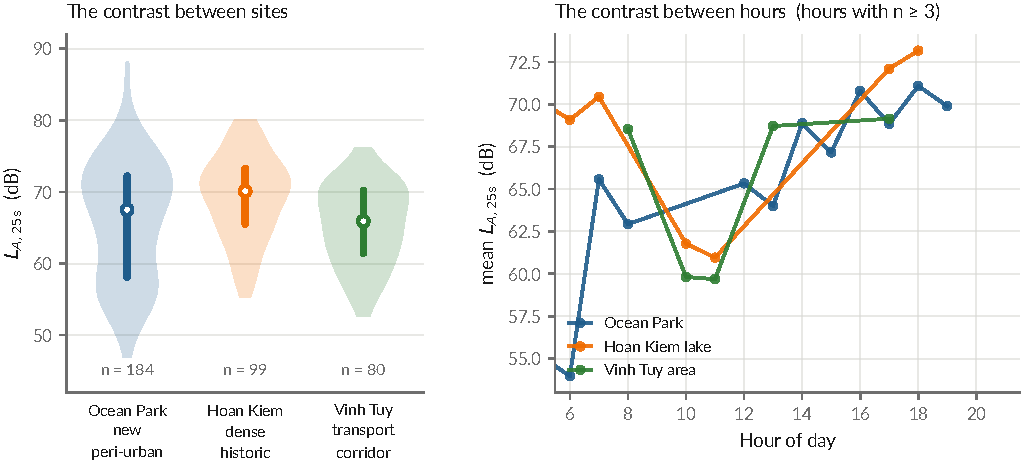
\includegraphics[width=.95\textwidth]{campaign.pdf}
  \caption{The 363 measurements: spatial layout, level distribution and temporal
  coverage. Produced by \pth{scripts/12\_presentation\_figures.py} from
  \pth{data/processed/measurements.csv} and \pth{models/metrics.json}.}
\end{figure}

\begin{center}\small
\begin{tabular}{@{}lrrrrrr@{}}
\toprule
\textbf{Site} & \textbf{$n$} & \textbf{mean} & \textbf{median} & \textbf{min} &
\textbf{max} & \textbf{$>$70\dB{} (day)} \\
\midrule
Ocean Park (new development)     & 184 & 65.9 & 67.5 & 47.0 & 88.0 & 35.6\,\% \\
Hoan Kiem lake (old quarter)     &  99 & 69.3 & 70.1 & 55.4 & 80.0 & 50.5\,\% \\
Vinh Tuy area (transport corridor) & 80 & 65.4 & 65.9 & 52.7 & 76.0 & 26.2\,\% \\
\midrule
All                              & 363 & 66.7 & 68.0 & 47.0 & 88.0 & 37.4\,\% \\
\bottomrule
\end{tabular}
\end{center}

\noindent\small Levels in \LAt{}. Computed from
\pth{data/processed/measurements.csv}; the exceedance column is the daytime
(06:00--21:00, $n=353$) proportion above the QCVN~26:2010 daytime value, as a
descriptive statistic and not as a compliance rate. Per-site exceedances from
\pth{results/tables/hanoi\_exceedances.csv}. Mean level peaks at hour~18
(71.7\dB).\normalsize

\subsection{Result 1 --- a three-parameter physical law beats every learned model}

The delivered model treats each road class as an incoherent line source, whose
intensity falls as $1/d$ rather than $1/d^{2}$:
\[
E(x) = \frac{A_{\mathrm{hw}}}{\max(d_{\mathrm{hw}}, d_0)}
     + \frac{A_{\mathrm{res}}}{\max(d_{\mathrm{res}}, d_0)} + B,
\qquad L(x) = 10\log_{10} E(x)
\]
with $d_{\mathrm{hw}}$ and $d_{\mathrm{res}}$ the distances to the nearest major
axis and to the nearest local street, separated by OSM \pth{highway} tag. Fitted
values (\pth{models/metrics.json}, \pth{physical\_params}):
$A_{\mathrm{hw}} = 4.774\times10^{7}$,
$A_{\mathrm{res}} = 3.800\times10^{7}$,
$B = 1.106\times10^{-10}$, $d_0 = 5$\,m; residual s.d.\ 6.07\dB.

\begin{center}\footnotesize
\begin{tabular}{@{}lccc@{}}
\toprule
\textbf{Model} & \textbf{Block-CV 600\,m} & \textbf{Buffered LOO 300\,m} &
\textbf{Leave-one-site-out} \\
\midrule
Mean by (site, hour)                & $-0.008$ & $-0.419$ & $-0.058$ \\
Regression on $\log d_{\text{road}}$ (2 par.) & 0.221 [0.09, 0.29] & 0.200 [0.08, 0.27] & 0.189 [0.06, 0.27] \\
\textbf{Physical kernel (3 par.) --- delivered} & 0.255 [0.09, 0.36] & \textbf{0.246 [0.10, 0.34]} & \textbf{0.222 [0.05, 0.33]} \\
LightGBM v1 (6 features)            & 0.304 [0.10, 0.46] & 0.137 [$-0.10$, 0.33] & 0.029 [$-0.35$, 0.21] \\
LightGBM v2 (8 features)            & 0.332 [0.11, 0.49] & 0.099 [$-0.13$, 0.25] & $-0.035$ [$-0.40$, 0.16] \\
Hybrid, physics + ML residual       & \textbf{0.395 [0.18, 0.53]} & 0.123 [$-0.22$, 0.29] & 0.035 [$-0.41$, 0.23] \\
Hybrid, capacity-restricted residual & 0.378 [0.20, 0.51] & 0.144 [$-0.15$, 0.35] & 0.106 [$-0.27$, 0.27] \\
\bottomrule
\end{tabular}
\end{center}

\noindent\small $R^2$ with 95\,\% block-bootstrap intervals, $n = 363$, 17
blocks, 2\,000 replicates. All values from \pth{models/metrics.json} via
\pth{models/model\_comparison.md}. Best per column in bold.\normalsize

\medskip
\textbf{The point of the table is the inversion.} Read the first column and the
hybrid leads; read the third and it is nearly worthless. The ranking reverses
monotonically as the split begins to test generalisation --- the signature of
capacity fitting spatial autocorrelation rather than physics. Three further
readings hold:

\begin{itemize}
  \item \textbf{The 300\,m morphological aggregates have negative marginal
        value.} Adding built-area ratio, road density and intersection count to
        distance-to-road \emph{degrades} prediction, by 0.07 $R^2$ under
        block-CV, 0.16 under buffered LOO and 0.18 under leave-one-site-out.
  \item \textbf{What remains of the ML model is time, not morphology.} The gap
        between the full model and the morphology-only ablation under block-CV
        (0.304 vs 0.153) is carried by the hour features. Under
        leave-one-site-out the time-only ablation is itself negative
        ($-0.139$).
  \item \textbf{The hybrid was built, tested and rejected}, not deferred. Against
        the bare physical core it gains $\Delta R^2 = +0.140$ under block-CV and
        loses $-0.123$ and $-0.187$ under the two strict protocols. The learned
        residual is computed at every run and deliberately not applied
        (\pth{apply\_residual: false}).
\end{itemize}

\begin{figure}[htbp]
  \centering
  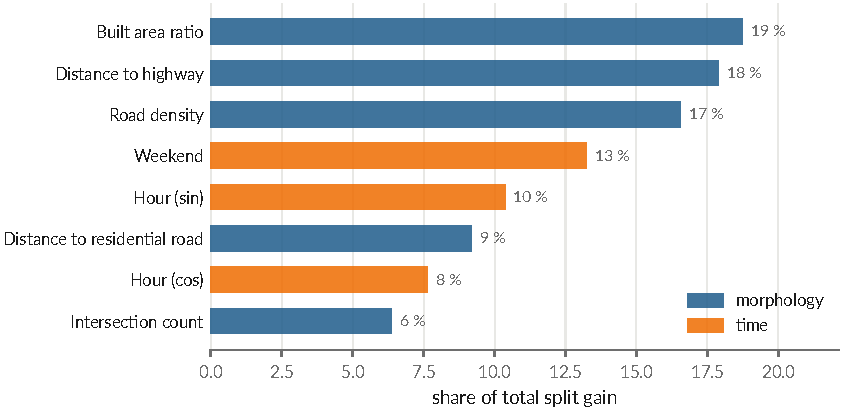
\includegraphics[width=.80\textwidth]{feature-importance.pdf}
  \caption{Gain-based feature importance inside the fitted LightGBM, kept because
  it explains the ablation: distance to road is the single largest contributor
  and matches the three area-aggregated descriptors combined.
  \pth{scripts/12\_presentation\_figures.py}.}
\end{figure}

\begin{figure}[htbp]
  \centering
  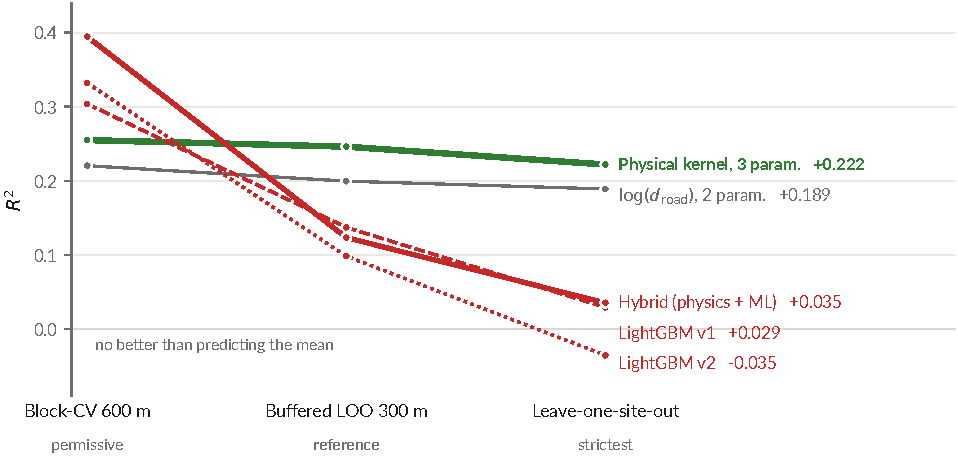
\includegraphics[width=.90\textwidth]{ranking-inversion.pdf}
  \caption{The ranking inversion, drawn. Same models, same folds, three
  protocols of increasing severity. \pth{scripts/12\_presentation\_figures.py}.}
\end{figure}

\begin{figure}[htbp]
  \centering
  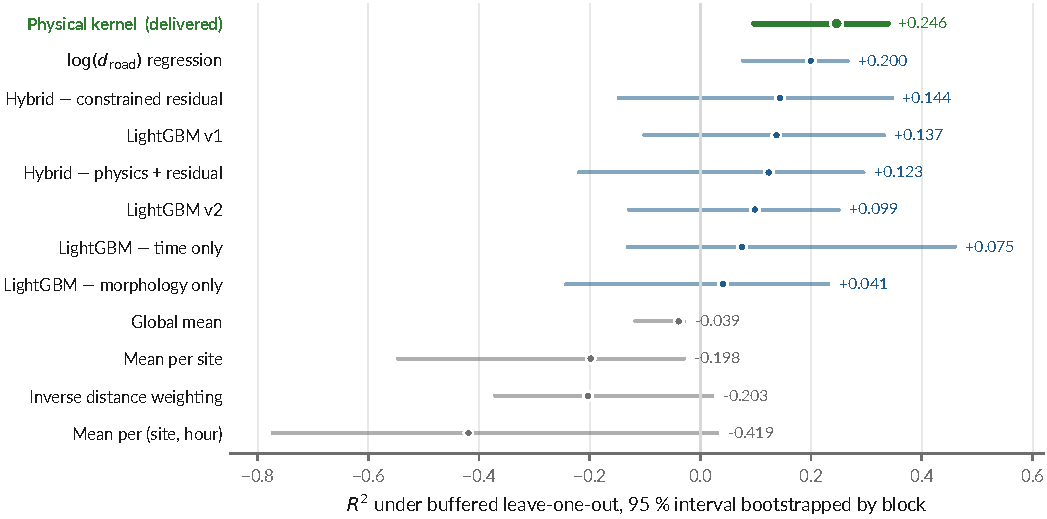
\includegraphics[width=.90\textwidth]{forest-bloo.pdf}
  \caption{Every model under the reference protocol with its 95\,\% interval.
  The physical kernel is the only model whose interval excludes zero under all
  three protocols --- and its interval overlaps that of the two-parameter
  distance regression almost entirely (§\ref{sec:ci}).}
\end{figure}

\subsection{Result 2 --- cross-city transfer fails, in three distinct ways}

Re-run for this report on \textbf{24 August 2026} with
\pth{scripts/experiments/uganda\_transfer.py}. It needs no Ugandan data: the two
Uganda boosters are versioned in \pth{models/}, and it evaluates them against
Hanoi's own 363 points.

\begin{center}\small
\begin{tabular}{@{}lcccc@{}}
\toprule
\textbf{Pretrained model} & \textbf{as delivered} & \shortstack{\textbf{mean diff.}\\\textbf{removed}} &
\shortstack{\textbf{and rescaled}\\\textbf{($=r^2$)}} & \textbf{$r$} \\
\midrule
Uganda 61K (v1)                   & $R^2 = -15.86$ & $-2.14$ & $+0.141$ & $\mathbf{-0.376}$ \\
Uganda convention-invariant (v2)  & $R^2 = -8.17$  & $-0.95$ & $+0.006$ & $+0.076$ \\
\midrule
\multicolumn{5}{@{}l}{\emph{For scale, fitted locally on the same 363 points:}} \\
$\log(\text{distance to road})$ alone & \multicolumn{4}{l}{$R^2 = +0.240$ (in sample)} \\
Physical kernel, buffered LOO         & \multicolumn{4}{l}{$R^2 = +0.246$} \\
\bottomrule
\end{tabular}
\end{center}

\begin{itemize}
  \item \textbf{It is not a calibration offset.} The Kampala model predicts about
        26\dB{} below Hanoi (MAE 26.5\dB, bias $-26.4$\dB), and removing that
        difference still leaves $R^2$ negative. A recalibrated transfer would not
        work either.
  \item \textbf{v1 transfers anti-information.} Its correlation with Hanoi is
        \emph{negative}: it ranks quiet and loud the wrong way round. The only way
        to extract anything from it is to flip it.
  \item \textbf{v2 removes the mapping-convention artefact and leaves nothing.}
        $r = +0.076$; even granted a free bias and a free slope its ceiling is
        $R^2 = 0.006$. Not wrong --- empty.
\end{itemize}

\noindent\textbf{One locally fitted distance term carries more than a
61\,000-point model trained in another city carries at all.}

\begin{caveat}{A small drift against the August brief}
\pth{docs/presentation-brief.md} §2.3 records $-15.8 / -2.17 / +0.151 / r=-0.388$
for v1 and $-8.1 / -0.96 / +0.004 / r=+0.066$ for v2. Today's rerun gives the
values tabulated above. The differences are small but not pure rounding.
\tc{whether the brief was computed at an earlier commit, or the experiment has a
non-deterministic component}. The manuscript must quote one run and name it.
\end{caveat}

\subsection{Result 3 --- vehicle counts from video carry no recoverable acoustic signal}

147 videos were matched to measurements (median offset 15\,s, p90 56\,s, max
161\,s). A non-negative least-squares regression in \emph{energy},
$E_{\text{total}} = E_{\text{background}(s)} + \sum_c n_c e_c$ with $e_c \ge 0$,
returns \textbf{exactly zero} for motorcycles and cars, in both passes:
per-frame density first, then --- after implementing the project's own
recommendation --- ByteTrack line-crossing flow.

Pooled over the 147 matched videos, total flow against measured level gives
$r = -0.109$ and motorcycle flow $r = -0.004$ (recomputed from
\pth{data/processed/vehicle\_counts.csv}). The one structured exception is Vinh
Tuy, the transport corridor, the only site with a positive association, which
\emph{strengthens} when density is replaced by flow ($r: +0.22 \to +0.30$).

The diagnosis in \pth{docs/negative-results.md} §5.x is that the failure is a
mismatch between the quantity measured and the quantity that governs the physics:
density is a stock and emission is driven by flow; speed dominates above
30--40\,km/h and is unobservable in a frame count; parked vehicles are counted;
and distance is discarded because the field of view is not georeferenced.

\begin{caveat}{This result should be reframed before submission}
The August data audit (recorded in \pth{presentation/main.tex}, slide
``Findings 2 and 3'') found the detector's modal split to be \textbf{57\,\% cars
and 36\,\% motorcycles} by density --- reproduced exactly from
\pth{vehicle\_counts.csv} for this report --- in a city where reality is roughly
the inverse. The matched subset also spans 61--80\dB{} against 47--88\dB{}
overall, cutting the standard deviation by 42\,\% (4.12 against 7.15\dB). A
negative correlation between traffic and noise is not physical. The audit's own
conclusion is that this is far more likely an \textbf{instrument failure than a
finding about acoustics}, and that it should be reported as ``the chain could not
be made to work''. \emph{The current wording in \pth{docs/negative-results.md}
has not yet been changed to match.}
\end{caveat}

\subsection{How good can any spatial model be here?}\label{sec:ceiling}

$R^2 \approx 0.25$ invites the question, so the project answers it with a
ceiling. Two measurements taken close together \emph{at the same hour} must be
predicted identically by any spatial model, so whatever they disagree by is
variance no spatial model can explain. Recomputed for this report from
\pth{measurements.csv}:

\begin{center}\small
\begin{tabular}{@{}lrrrr@{}}
\toprule
\textbf{Separation} & \textbf{Pairs} & \textbf{Mean $|$difference$|$} &
\textbf{Implied $\sigma$} & \textbf{Ceiling on $R^2$} \\
\midrule
$<20$\,m & 29  & 4.23\dB & 3.75\dB & 0.72 \\
$<40$\,m & 87  & 5.44\dB & 4.82\dB & \textbf{0.54} \\
$<60$\,m & 229 & 6.09\dB & 5.40\dB & 0.43 \\
\bottomrule
\end{tabular}
\end{center}

\noindent\small Conversion: for two readings of a common value with error s.d.
$\sigma$, the difference is $N(0, 2\sigma^2)$, so
$\sigma = \overline{|{\Delta}|}\sqrt{\pi}/2$. Total variance of the 363
measurements is 51\dB$^2$.\normalsize

\medskip
At the 40\,m scale the map works at, the ceiling is around $R^2 \approx 0.54$.
The delivered model reaches 0.246 --- about half of what is attainable, not a
tenth of it. \textbf{The caveat belongs on the same page}: pairs at the same hour
may fall on different days, so this $\sigma$ carries day-to-day variation and
overestimates pure measurement noise; and 29 pairs is few. It is an order of
magnitude, not a bound.

\begin{figure}[htbp]
  \centering
  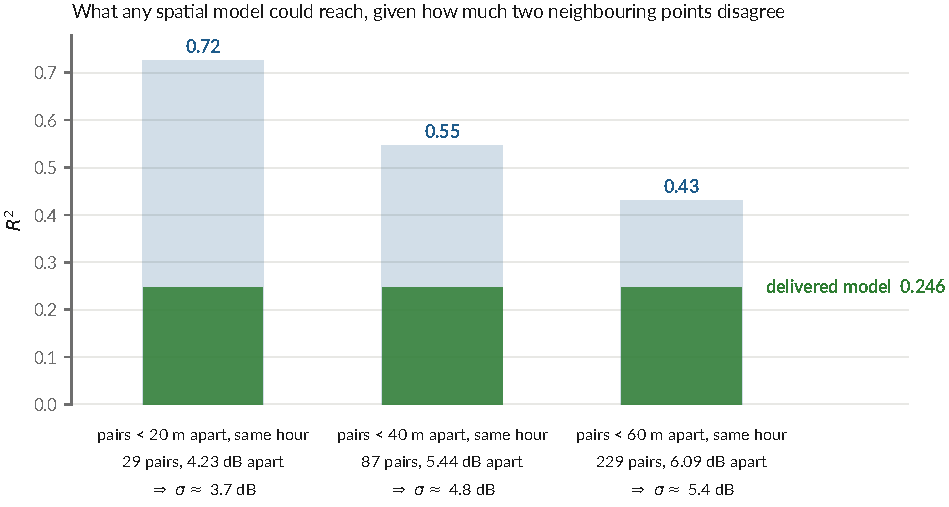
\includegraphics[width=.86\textwidth]{ceiling.pdf}
  \caption{The ceiling, drawn. \pth{scripts/12\_presentation\_figures.py}.}
\end{figure}

\subsection{The published map and the simulation}

The exported grid is 5\,587 cells at 40\,m over three zones $\times$ 17 hours
(\pth{results/maps/hanoi\_noise\_map.csv}), and it covers the sampled envelope
only --- the three measured sites plus a 400\,m margin.

\begin{figure}[htbp]
  \centering
  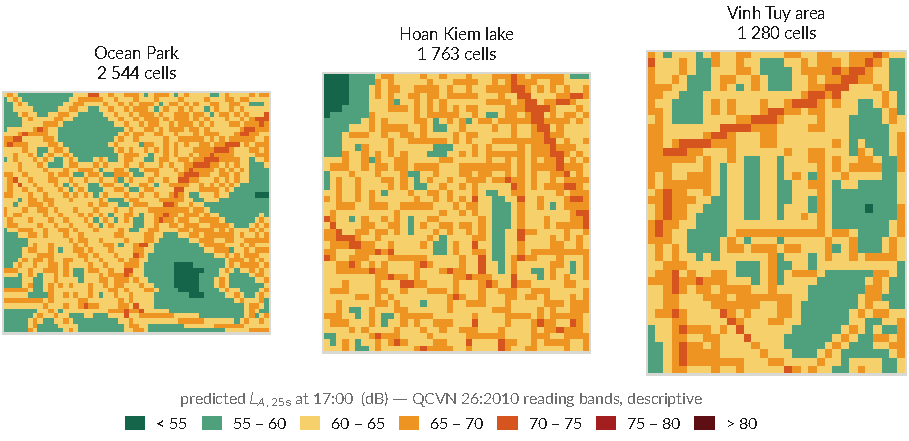
\includegraphics[width=.92\textwidth]{map-grid.pdf}
  \caption{The published 40\,m grid, redrawn from the CSV rather than
  screenshotted. QCVN 26:2010 colour bands, used descriptively.}
\end{figure}

\begin{figure}[htbp]
  \centering
  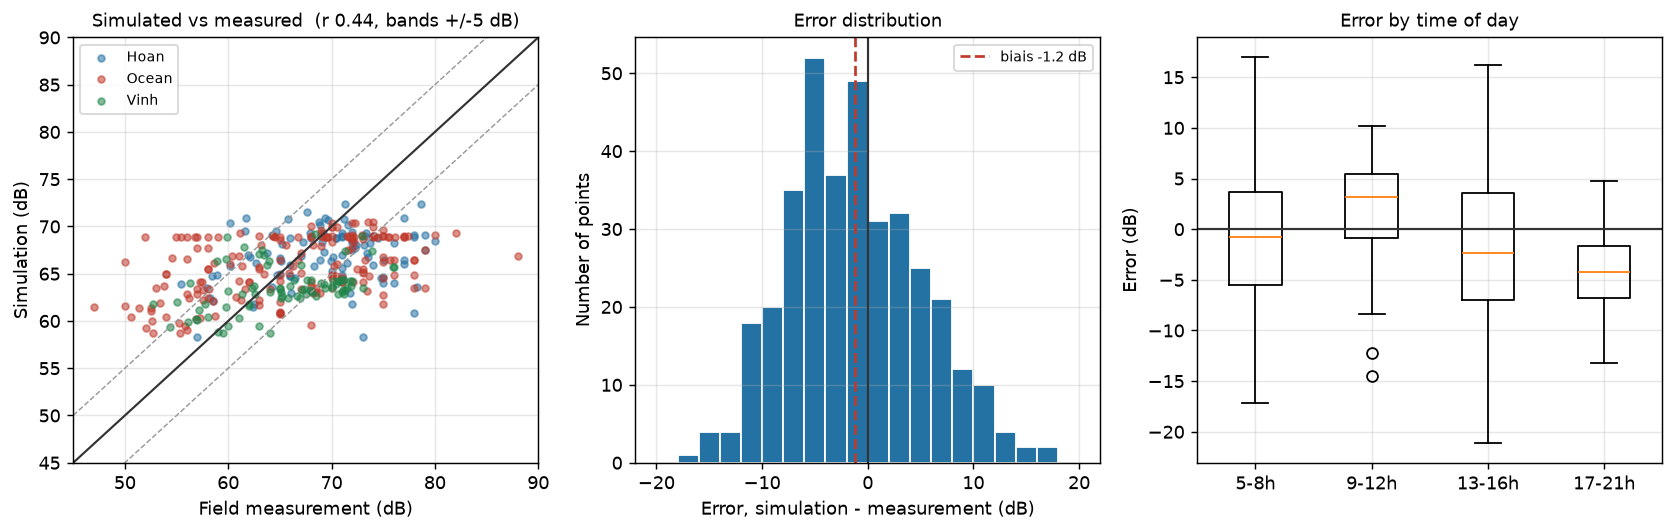
\includegraphics[width=.80\textwidth]{validation_simulation.png}
  \caption{Simulated against measured levels, $n = 360$ matched points
  (\pth{results/tables/validation\_simulation.csv},
  \pth{scripts/08\_validate\_simulation.py}). Mean error $-1.24$\dB, MAE
  5.30\dB, RMSE 6.49\dB. The simulation reproduces the spatial and temporal
  ordering; it does not reproduce the spread, which is expected given that
  features aggregated over 300\,m cannot resolve the facade/courtyard contrast.}
\end{figure}

\begin{caveat}{This validation was itself a lesson}
An earlier published validation reported MAE 3.79\dB. It had validated a grid
that was regenerated after it, and the drift was found on 11 August by re-running
the script during an unrelated task --- not by any check. The flattering figures
were the stale ones. The old artefact is archived with its reason
(\pth{docs/archive/validation-2026-08-05/}) and the Makefile now declares the
dependency so \pth{make} rebuilds it.
\end{caveat}

\subsection{What could not be regenerated}

Eight figures in \pth{results/figures/sunbird/} --- the Uganda reproduction ---
are frozen images that never had a scripted producer: they come from notebook
cells whose input data is absent from the repository. They are marked as such
(\pth{NOT-REGENERABLE.md}) rather than quietly reused. One of them,
\pth{pred\_vs\_real.png}, carries ``$R^2 = 0.250$'' for the \emph{Uganda}
reproduction, which is easily mistaken for the Hanoi delivered model's 0.246; the
two are unrelated. \textbf{No such figure is used in this report.}

% ============================================================================
\section{Discussion, limitations and open questions}

\subsection{The two limits that are not fixable by code}

\paragraph{No absolute reference.} Three handsets were cross-calibrated against
each other and against no standard, so every level in this project is relative.
\pth{docs/metrology.md} argues this well, but a reviewer in acoustics will ask
whether one afternoon beside a class~1 or class~2 meter was truly out of reach.
It would convert ``calibrated in relative terms'' into ``calibrated'' and would
open the comparisons the work currently forbids itself.

\paragraph{Three sites are three typologies.} The effective number of independent
morphological configurations is close to three whatever the number of points, and
three is not a basis for claiming coverage of a city. This bounds generalisation
further than the $R^2$ does, and it is the reason every published map stops at
the sampled envelope.

\subsection{The open finding: a $-5$\dB{} discontinuity on 27 June}

This is, in my assessment, the most serious unresolved item, and it is
\textbf{not yet written up anywhere in \pth{docs/}} --- it exists only in the
August deck (\pth{presentation/main.tex}, frame ``Finding 1'') and in
\pth{scripts/12\_presentation\_figures.py}.

Verified from \pth{measurements.csv} for this report: the mean level before
27~June is 69.75\dB{} ($n=148$) and after it 64.66\dB{} ($n=215$), a raw gap of
$-5.09$\dB. On the same date the share of integer-valued readings falls from
\textbf{87\,\% to 20\,\%}, which is the signature of a change in the recording
instrument or form rather than of the city getting quieter.

\begin{figure}[htbp]
  \centering
  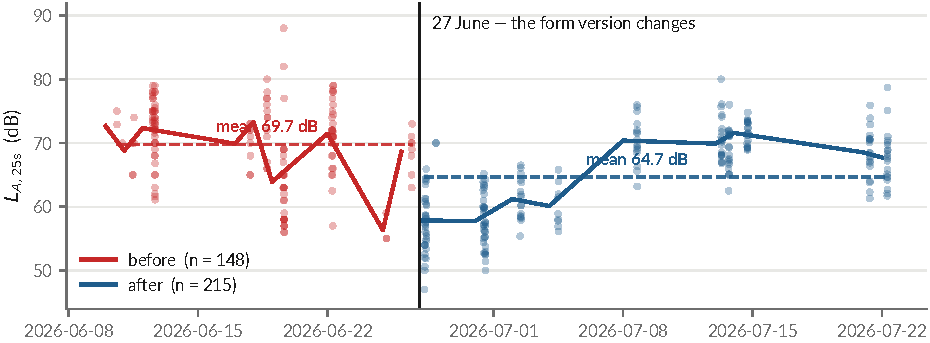
\includegraphics[width=.90\textwidth]{discontinuity.pdf}
  \caption{The level distribution around 27 June 2026. The break date is not
  chosen by the figure: it is the date the form version changes. Produced by
  \pth{scripts/12\_presentation\_figures.py} from
  \pth{data/processed/measurements.csv}.}
\end{figure}

The deck reports a controlled effect of $-5.14$\dB{} (SE 0.55,
$p \approx 10^{-20}$) and states that before/after is predictable from
$(\mathrm{lat}, \mathrm{lon})$ alone at AUC~0.83 --- so an instrumental shift is
\emph{spatially structured}, and a model can learn it as morphology.

\begin{caveat}{What I could and could not reproduce}
The raw gap and the integer-reading collapse reproduce exactly. The
\emph{controlled} $-5.14$\dB{} does not: no script in the repository computes it,
so the specification behind it (which covariates, which encoding) cannot be
recovered. Refitting with site, class and hour dummies gives $-7.75$\dB{}
(SE 0.71) --- same sign, same order, different number.
\tc{the exact specification behind the $-5.14$\dB{} figure, and where its code
lives}. Until the code exists in the repository, neither figure should go in the
manuscript.
\end{caveat}

\noindent The buffered leave-one-out protocol excludes 300\,m around each test
point. \textbf{It does not exclude a period.} That is the gap, and the indicated
fix is to diagnose the cause and refit with a phase term.

\subsection{The headline ranking is not statistically separated}\label{sec:ci}

Physical kernel $R^2 = 0.246$, CI $[0.097, 0.339]$, against
$\log d_{\text{road}}$ at $0.200$, CI $[0.077, 0.266]$. The intervals overlap
almost entirely. ``The physical kernel beats log-distance'' is, on this sample, a
coin flip. What survives is the stronger and better-supported claim: \emph{both
simple geometric models beat every learned model under every protocol that tests
generalisation, and they are the only models that barely move between
protocols.} Every summary table in the manuscript must carry the intervals.

\subsection{Other known weaknesses}

\begin{itemize}
  \item \textbf{The vehicle detector has never been validated} against manual
        counts. Precision, recall and MAPE per class are unknown, and
        two-wheeler under-detection is expected but unquantified. \emph{Modal
        shares must not be published until it is.} One day of manual counting on
        ten videos turns an open-ended limitation into a quantified uncertainty.
  \item \textbf{The Uganda chain (notebooks 01--06) is not reproducible} on a
        fresh machine: it expects \pth{data/processed/uganda/*}, which exists
        nowhere. The transfer \emph{experiment} is now reproducible from the
        versioned boosters, but the pretraining is not.
  \item \textbf{Night is not sampled.} 10 measurements fall outside 06:00--21:00
        and there are none between 22:00 and 03:00.
  \item \textbf{15\,\% of \pth{construction\_nearby} is inferred} from the noise
        class rather than observed, and the published CSV does not flag observed
        against derived values.
  \item \textbf{Technical debt}: \pth{04\_evaluate\_models.py} is 598 lines
        holding three CV protocols, the bootstrap and six model definitions ---
        the most valuable code in the project is the least testable;
        \pth{07\_export\_gama\_inputs.py} is 414 lines doing five jobs.
\end{itemize}

\subsection{Inconsistencies found while writing this report}

Small, but each one contradicts the project's own single-source rule, and each is
a five-minute fix:

\begin{enumerate}
  \item \textbf{The test suite does not currently pass.} In
        \pth{tests/test\_pipeline\_end\_to\_end.py},\\
        \pth{test\_every\_pipeline\_step\_is\_present}
        asserts scripts \pth{01}--\pth{11}, and script \pth{12} was added on
        21~August (\pth{eb9c349}). Actual state on 24 August 2026:
        \textbf{41 passed, 1 failed, 1 deselected}.
  \item \textbf{The README badge says ``34 tests''}; the suite collects 42.
  \item \textbf{The README's night claim is wrong in both halves.} It says ``10
        measurements after 21:00, none 00:00--05:00''. In fact one measurement is
        at hour~21 and nine are at hours 4--5. The count of 10 is right; the
        window is not.
  \item \textbf{One exceedance figure lives in two places and they disagree}:
        \pth{docs/literature-review.md} says 38.6\,\%,
        \pth{results/report/numbers.tex} says 37.4\,\%. The data gives 37.4\,\%
        for daytime samples above 70\dB.
  \item \textbf{The transfer numbers in the presentation brief do not match
        today's rerun} (§4.3).
  \item \textbf{The August data-audit findings are not in \pth{docs/}.} The deck
        cites \pth{docs/audit/} for the 27~June discontinuity; that directory
        contains the 5~August scientific audit and the restructuring documents,
        not this one.
\end{enumerate}

% ============================================================================
\section{Next steps and timeline}

Dates are the repository's where it has them, and marked otherwise where it does
not.

\subsection{Blocking before any public release}

\begin{enumerate}
  \item \textbf{Confirm the host affiliation} --- CEI or COSMOS Lab. The June
        2026 survey says \emph{Center for Environmental Intelligence}; the team
        was told \emph{COSMOS Lab}. They may nest rather than conflict.
        Placeholders sit in \pth{CITATION.cff}, \pth{docs/handover.md} and
        \pth{docs/data-sources.md}. \emph{Holder of the answer: supervisor /
        VinUniversity.}
  \item \textbf{Video retention decision} --- custodian, storage location,
        deletion or anonymisation deadline. 6\,GB of unanonymised video showing
        faces and plates currently sits with no owner and no expiry. This is the
        most consequential open item in the project. \emph{Holder: supervisor.}
  \item \textbf{Identity metadata} --- Lucas Zborowski's ORCID; Doanh
        Nguyen-Ngoc's title; whether Nguyen Thanh Quang is a co-author or an
        acknowledgement (the current default is \emph{contributor} plus
        acknowledgement).
  \item \textbf{Ownership of the KoboToolbox account} if the app is used for a
        public campaign --- it should be institutional, not a student's, because
        whoever owns it holds strangers' GPS positions and timestamps. And
        \textbf{VinUniversity ethics review} before any new collection: the video
        collection went without one and the repository says so; that must not be
        repeated at larger scale.
\end{enumerate}

\subsection{Scientific work, in value-per-effort order}

\begin{enumerate}
  \item \textbf{Validate the YOLO detector} on \(\sim\)10 videos, double-counted
        manually --- about one day. It is the input uncertainty of every
        downstream number and it unblocks the modal shares.
  \item \textbf{Diagnose the 27~June discontinuity} and refit with a phase term
        --- and commit the code that computes the controlled effect.
  \item \textbf{Reframe negative result 3} as an instrument failure in
        \pth{docs/negative-results.md} and in the manuscript.
  \item \textbf{Carry the confidence intervals into every summary table.}
  \item \textbf{Implement a real propagation kernel} --- CNOSSOS-EU via
        NoiseModelling \citep{kephalopoulos2014cnossos, bocher2019noisemodelling}.
        This is the scientifically indicated continuation, not an optional
        extra: if a two-parameter distance term already beats a six-variable
        gradient-boosting model, then physical propagation corrected by a locally
        learned residual is the architecture the data points at. It was out of
        budget for a three-month internship; implementing it is months, citing
        what is missing is a page.
  \item \textbf{Repeat a short campaign with a reference instrument} to anchor
        the absolute scale. The app's calibration screen exists for exactly this.
\end{enumerate}

\subsection{Deliverable track}

\begin{center}\small
\begin{tabular}{@{}p{4.2cm}p{4.2cm}p{5.4cm}@{}}
\toprule
\textbf{Deliverable} & \textbf{State} & \textbf{Next action} \\
\midrule
Manuscript (Overleaf) & Two sections drafted in the repository first
  (\pth{metrology.md}, \pth{negative-results.md}); Overleaf is the source of
  truth & Reframe result 3; add the intervals; add the CNOSSOS future-work
  paragraph with Figure~2 of \citet{bocher2019noisemodelling}; resolve the
  byline. \tc{target venue and date} \\
Capture / demo with the app & Working end to end; the three-gesture demo is
  scripted in \pth{docs/presentation-brief.md} §5 & Record it. Steps 1--2
  (measurement, map) need no network; step 3 (GAMA) needs
  \pth{gama-headless.sh -socket 6868} reachable on the wifi address, not
  localhost. \tc{date} \\
AAMAS submission or presentation & \textbf{Nothing in the repository mentions
  AAMAS} --- no deadline, no venue, no track & \tc{venue, track (full paper /
  extended abstract / demo), and deadline}. The agent-based exposure model
  (\pth{simulation/gama/}) is the natural hook; tier~2 pedestrian agents are the
  natural addition. \\
Decks & 35-slide and 23-slide versions compiled, plus speaker scripts and a
  formula annex (\pth{presentation/}) & Ready. \\
\bottomrule
\end{tabular}
\end{center}

\subsection{Deliberately abandoned}

LSTM / ST-GNN benchmarking on Barcelona (those models need continuous time
series this campaign does not produce; \pth{barcelona\_transfer.py} is kept as a
documented dead end); emitter agents in GAMA; demolition audio; per-class vehicle
emission coefficients. \textbf{Acoustic event localisation} --- the ``gunshot''
direction --- is a different project rather than a continuation: time-difference-
of-arrival localisation needs clocks agreeing to about 35\,ms for a $\pm$12\,m
fix, continuous listening, and at least four sensors at known fixed positions.
This campaign has 363 spot measurements from three unsynchronised handsets. It is
strong as future work and wrong as a promise attached to this result.

% ============================================================================
\appendix
\clearpage
\section{Register of unconfirmed items}

\begin{center}\small
\begin{longtable}{@{}p{4.6cm}p{5.2cm}p{4.0cm}@{}}
\toprule
\textbf{Item} & \textbf{Why it is open} & \textbf{Who holds the answer} \\
\midrule
\endhead
Author's exact internship dates & The repository dates the work only by commit
  (1 June --- 21 August 2026) and by the field campaign (10 June --- 22 July
  2026) & The author / the host institution \\
Host laboratory: CEI or COSMOS Lab & The June 2026 survey says \emph{Center for
  Environmental Intelligence}; the team was told \emph{COSMOS Lab} & Supervisor /
  VinUniversity \\
Doanh Nguyen-Ngoc's title & Placeholder in \pth{CITATION.cff} and the title
  slide & Doanh Nguyen-Ngoc \\
Lucas Zborowski's ORCID & Placeholder in \pth{CITATION.cff} & Lucas Zborowski \\
Nguyen Thanh Quang: co-author or acknowledgement & Currently \emph{contributor}
  plus acknowledgement --- the default that wrongs nobody & Nguyen Thanh Quang \\
Video retention: custodian, location, deletion deadline & 6\,GB of unanonymised
  video with no owner and no expiry & Supervisor \\
Publication status of the June 2026 survey & Marked \pth{[À VÉRIFIER]}; PDF
  withdrawn from \pth{HEAD} because it carries personal e-mail addresses & The
  two authors \\
AAMAS venue, track and deadline & \textbf{No mention of AAMAS anywhere in the
  repository} & The supervisor / the author \\
Recipients of this report & No e-mail address for the supervisor or for
  ``Phung'' appears anywhere in the repository & The author \\
Specification behind the $-5.14$\dB{} controlled discontinuity & No script in the
  repository computes it & Whoever ran the August data audit \\
Whether the transfer brief was computed at an earlier commit & Today's rerun
  differs slightly (§4.3) & Whoever ran it \\
Twelve journal quartiles & Scimago returns HTTP 403 to automated requests; a
  search engine's summary is second-hand & 15 minutes in a browser \\
\citet{phan2010characteristics} $L_\mathrm{den}$ values & Currently from
  secondary sources, flagged \pth{to\_check} & The PDF, via the VinUniversity
  library \\
Author list of \citet{anh2024motorcycle} & \pth{[AUTHORS TO CONFIRM]} in the
  \pth{.bib} & The article \\
\bottomrule
\end{longtable}
\end{center}

\section{Provenance of every figure and recomputed number}

\begin{center}\small
\begin{tabular}{@{}p{4.4cm}p{9.4cm}@{}}
\toprule
\textbf{Artefact} & \textbf{Producer} \\
\midrule
\pth{campaign.pdf}, \pth{ranking-inversion.pdf}, \pth{forest-bloo.pdf},
\pth{ceiling.pdf}, \pth{map-grid.pdf}, \pth{discontinuity.pdf},
\pth{feature-importance.pdf}
  & \pth{scripts/12\_presentation\_figures.py}, reading
    \pth{models/metrics.json}, \pth{data/processed/measurements.csv} and
    \pth{results/maps/hanoi\_noise\_map.csv}. Re-run on 24 August 2026;
    output identical to the committed versions apart from PDF timestamps. \\
\pth{validation\_simulation.png} & \pth{scripts/08\_validate\_simulation.py} \\
Model table (§4.2) & \pth{models/metrics.json} via \pth{models/model\_comparison.md} \\
Transfer table (§4.3) & \pth{scripts/experiments/uganda\_transfer.py}, re-run 24 August 2026 \\
Site table, exceedances, hour peak, night counts & recomputed from
  \pth{data/processed/measurements.csv} and
  \pth{results/tables/hanoi\_exceedances.csv} \\
Ceiling table (§\ref{sec:ceiling}) & recomputed from
  \pth{data/processed/measurements.csv} \\
Modal split, match gaps, flow correlations & recomputed from
  \pth{data/processed/vehicle\_counts.csv} \\
Discontinuity raw gap and integer-reading share & recomputed from
  \pth{data/processed/measurements.csv} \\
Simulation validation statistics & recomputed from
  \pth{results/tables/validation\_simulation.csv} ($n=360$) \\
App statistics & counted in \pth{mobile/app/src/} \\
Test-suite state & \pth{pytest tests -q}, 24 August 2026 \\
\bottomrule
\end{tabular}
\end{center}

\clearpage
\bibliographystyle{plainnat}
\renewcommand{\refname}{References}
\bibliography{refs}

\end{document}
